%% LaTeX2e class for student theses
%% sections/content.tex
%% 
%% Karlsruhe Institute of Technology
%% Institute for Program Structures and Data Organization
%% Chair for Software Design and Quality (SDQ)
%%
%% Dr.-Ing. Erik Burger
%% burger@kit.edu
%% burger@kit.edu
%%
%% Version 1.3.3, 2018-04-17


\chapter{Untersuchung von nachrichtenbasierter Middleware}
\label{ch:mom}
Um die Performance einer MOM, oder eines Software-Systems im Allgemeinen, vorhersagen zu können, benötigt man zunächst Informationen über die Struktur des Systems, sein Verhalten, seine Ausführungsumgebung und über die Benutzung. Dazu müssen die verschiedenen Palladio-Rollen relevante Einflüsse bestimmen können. Der Komponenten-Entwickler muss Ressourcen-Anforderungen und Fehlerraten bestimmen. Der Software-Verteilungs-Experte muss verfügbare Rechenleistung und Hardware bestimmen. Der Domänenexperte muss das Verhalten der Nutzer bestimmen. Schließlich muss der Softwarearchitekt fehlende Werte bestimmen und das Modell damit kalibrieren. Diese Modellkalibrierung ist ein wichtiger Bestandteil des Modellierungsprozesses. In \cite{palladio17} wird beschrieben, wie und mit welchen Techniken die verschiedenen Rollen diese Daten erhalten und die jeweiligen Modelle kalibrieren können. Modellkalibrierung ist dabei die Anreicherung von Modellen mit quantitativen Daten, wie Ressourcenbedarf. Die Daten können aus Messungen oder Vorhersagen stammen. Die Modellkalibrierung ist eine Vorbedingung der Performance-Analyse. Die Informationen die eine Rolle in den verschiedenen Phasen der Software-Entwicklung gewinnen kann sind unterschiedlich. Dieser Prozess lässt sich in drei Aktivitäten strukturieren: Design, Entwicklung und Betrieb. Während der Design-Aktivität existiert die Applikation nur auf dem Papier und die Daten, die gesammelt werden können sind Schätzungen. Je weiter die Software-Entwicklung fortgeschritten ist, desto mehr quantitative Daten werden verfügbar um die Modelle kalibrieren zu können. Schließlich kann in der Betriebsphase das Gesamtsystem und auch der Benutzer quantitative Daten liefern. 

Im Rahmen der Masterarbeit wurde eine MOM modelliert um in Performance-Analysen eingesetzt werden zu können. Dazu wurden, wie oben beschrieben, verschiedenen Daten gesammelt um das Modell kalibrieren zu können, damit eine Performance-Analyse ermöglicht wird. Dazu wurde zunächst eine bereits existierende MOM ausgewählt. Da sie sich damit im letzten Schritt der drei Software-Entwicklungsaktivitäten befindet, konnte das Gesamtsystem betrachtet und ausgemessen werden, um quantitative Daten zu sammeln. Für die Auswahl wurden zunächst in \autoref{sec:anforderungenMom} Anforderungen an die MOM definiert. Die ausgewählte MOM wird im Anschluss in \autoref{sec:rmq} vorgestellt. Die Ergebnisse der Ausmessung der MOM sind in \autoref{sec:rmqBenchmark} beschrieben. Mithilfe der Ergebnisse, werden die Modelle in \autoref{ch:modellierung} anschließend kalibriert.


\section{Anforderungen an MOMs}
\label{sec:anforderungenMom}
Da es eine Vielzahl von MOMs gibt, muss zunächst eine Auswahl stattfinden. Dazu werden im ersten Schritt der Masterarbeit Anforderungen erarbeitet, die ein MOM erfüllen muss, damit sie in Betracht kommt. Die folgenden Anforderungen sollen erfüllt werden:
\begin{itemize}
\item Die MOM soll \textbf{Open Source} sein.
\item Sie soll eine \textbf{weite Verbreitung} haben.
\item Die Verwendung soll \textbf{Programmiersprachen unabhängig} sein.
\item Es soll eine MOM betrachtet werden, die sich in \textbf{aktiver Entwicklung} befindet.
\item Die verschiendenen \textbf{Interaktionstypen} (1:1, 1:n, n:1 und n:m) sollen unterstützt werden
\item Sie soll einen \textbf{hohen Grad der Entkopplung}, bzgl. Raum, Zeit und Synchronisation haben
\item Die MOM soll sowohl das Punkt-Zu-Punkt als auch Publish/Subscriber \textbf{Nachrichtenmodell} unterstüzen
\end{itemize}
%- bestimmte Protokolle unterstuetzen \\ %(https://www.predic8.de/activemq-hornetq-rabbitmq-apollo-qpid-vergleich.htm)

%\section{Auswahl der MOMs}
%In diesem Schritt sollen zwei bis drei MOMs ausgewählt werden. Dabei sollen die zuvor erarbeiteten Anforderungen einbezogen werden. Da sich bereits im Rahmen des Proposals mit dem Thema auseinander gesetzt wurde, wurden bereits drei starke Kandidaten identifiziert, die die bereits erarbeiteten Anforderungen erfüllen.
Im Folgenden soll eine MOM untersucht werden, das diese Anforderungen erfüllt.

\section{RabbitMQ}
\label{sec:rmq}
RabbitMQ (RMQ) ist, mit 35,000 aktiven Produktivumgebungen, eine der am weitesten verbreitete MOMs. 
RMQ ist Open-Source und wird seit 2007 immer weiter entwickelt \cite{rabbitmq}. Das Ziel von RMQ ist es, allgemein einsetzbar zu sein. Deshalb wird eine Vielzahl an Protokollen unterstützt, unter anderem das JMS-Protokoll. RMQ kann auf einem zentralen Konten oder auf mehreren verteilten Knoten eingesetzt werden. Für den Nachrichtenaustausch verwendet RMQ Warteschlangen. Diese lassen sich unterschiedlich konfigurieren, zum Beispiel in ihrer Warteschlangenlänge. Das Kommunizieren zwischen Sender und Empfänger geschieht dabei nicht direkt über die Warteschlange. Nachrichten werden zunächst an einen sogenannten \emph{Exchange} (dt. Austausch) gesendet. Dieser ist für das richtige Weiterleiten an die passende Warteschlange verantwortlich. Dies geschieht mit Hilfe von Bindungen und Routing-Schlüsseln. In RMQ ist eine Bindung eine Verbindung zwischen einer Warteschlange und einem Exchange. RMQ unterscheidet zwischen vier verschiedenen Exchange-Typen:
\begin{itemize}
    \item Direct: Hierbei meldet sich eine Warteschlange mit einem bestimmten Routing-Schlüssel X beim Exchange an. Wenn eine Nachricht mit einem Routing-Schlüssel Y ankommt, wird sie nur an die Warteschlange gesendet, wenn die Routing-Schlüssel X und Y übereinstimmen.
    \item Topic: Die Warteschlange ist mithilfe einer Bindung mit einem Exchange verbunden. Nachrichten werden wieder anhand des Routing-Schlüssels weitergeleitet. Der Routing-Schlüssel muss nicht mehr genau passen, sondern muss ein bestimmtes Muster aufweisen.
    \item Fanout: Die ankommende Nachricht wird an alle mit dem Exchange verbundenen Warteschlangen gesendet. Der Routing-Schlüssel wird dabei ignoriert.
    \item Header: Dabei werden die Attribute des Nachrichtenkopfes verwendet, um die Nachricht weiterzuleiten.
\end{itemize}
Diese Architektur erlaubt verschiedene Interaktionstypen. Sowohl eins-zu-eins als auch viele-zu-viele Interaktionen sind möglich. Dabei können nicht nur mehrere Warteschlangen existieren, sondern auch mehrere Exchanges und jede der Komponenten kann auf einem anderen Knoten verteilt sein. Aufgrund dieser Architektur hat RMQ auch einen hohen Grad der Entkopplung. Den Sender und Empfänger müssen sich nicht kennen, sie kommunizieren lediglich über den Exchange miteinander. Weder der Sender noch der Empfänger müssen zur gleichen Zeit aktiv sein. Der Sender sendet Nachrichten an die Warteschlange und der Empfänger entnimmt sie, wenn er die dazu nötigen Ressourcen zur Verfügung hat. Schließlich müssen Sender und Empfänger nicht aufeinander warten, da sie über eine Warteschlange kommunizieren.
In \autoref{img:rmq_architecture} ist ein Beispiel für eine mögliche RMQ-Architektur und Kommunikation zwischen Sendern und Empfängern dargestellt. Dabei ist \emph{ExchangeA} vom Typ Direkt. Dieser ist mit der \emph{Bestellungs}-Warteschlange verbunden. \emph{ExchangeB} ist ein Topic-Exchange und mit \emph{Bestätiguns}-Warteschlange und der \emph{Statistik}-Warteschlange verbunden. Dabei unterscheiden sich die beiden Bindungen in ihrem Routing-Muster. EmpfängerA empfängt Nachrichten aus der \emph{Bestellungs}-Warteschlange und EmpfängerB Nachrichten aus der \emph{Bestätiguns}- und \emph{Statistik}-Warteschlange. Wenn ein Sender eine Nachricht an \emph{ExchangeA} sendet, wird diese in der \emph{Bestellungs}-Warteschlange abgelegt, wenn der Routing-Schlüssel der Nachricht mit dem Routing-Schlüssel der Warteschlange übereinstimmt. Wenn eine Nachricht an ExchangeB gesendet wird, wird anhand des Routing-Musters entschieden, ob die Nachricht an die \emph{Bestätiguns}- oder \emph{Statistik}-Warteschlange gesendet wird. 
\begin{figure}
\center
  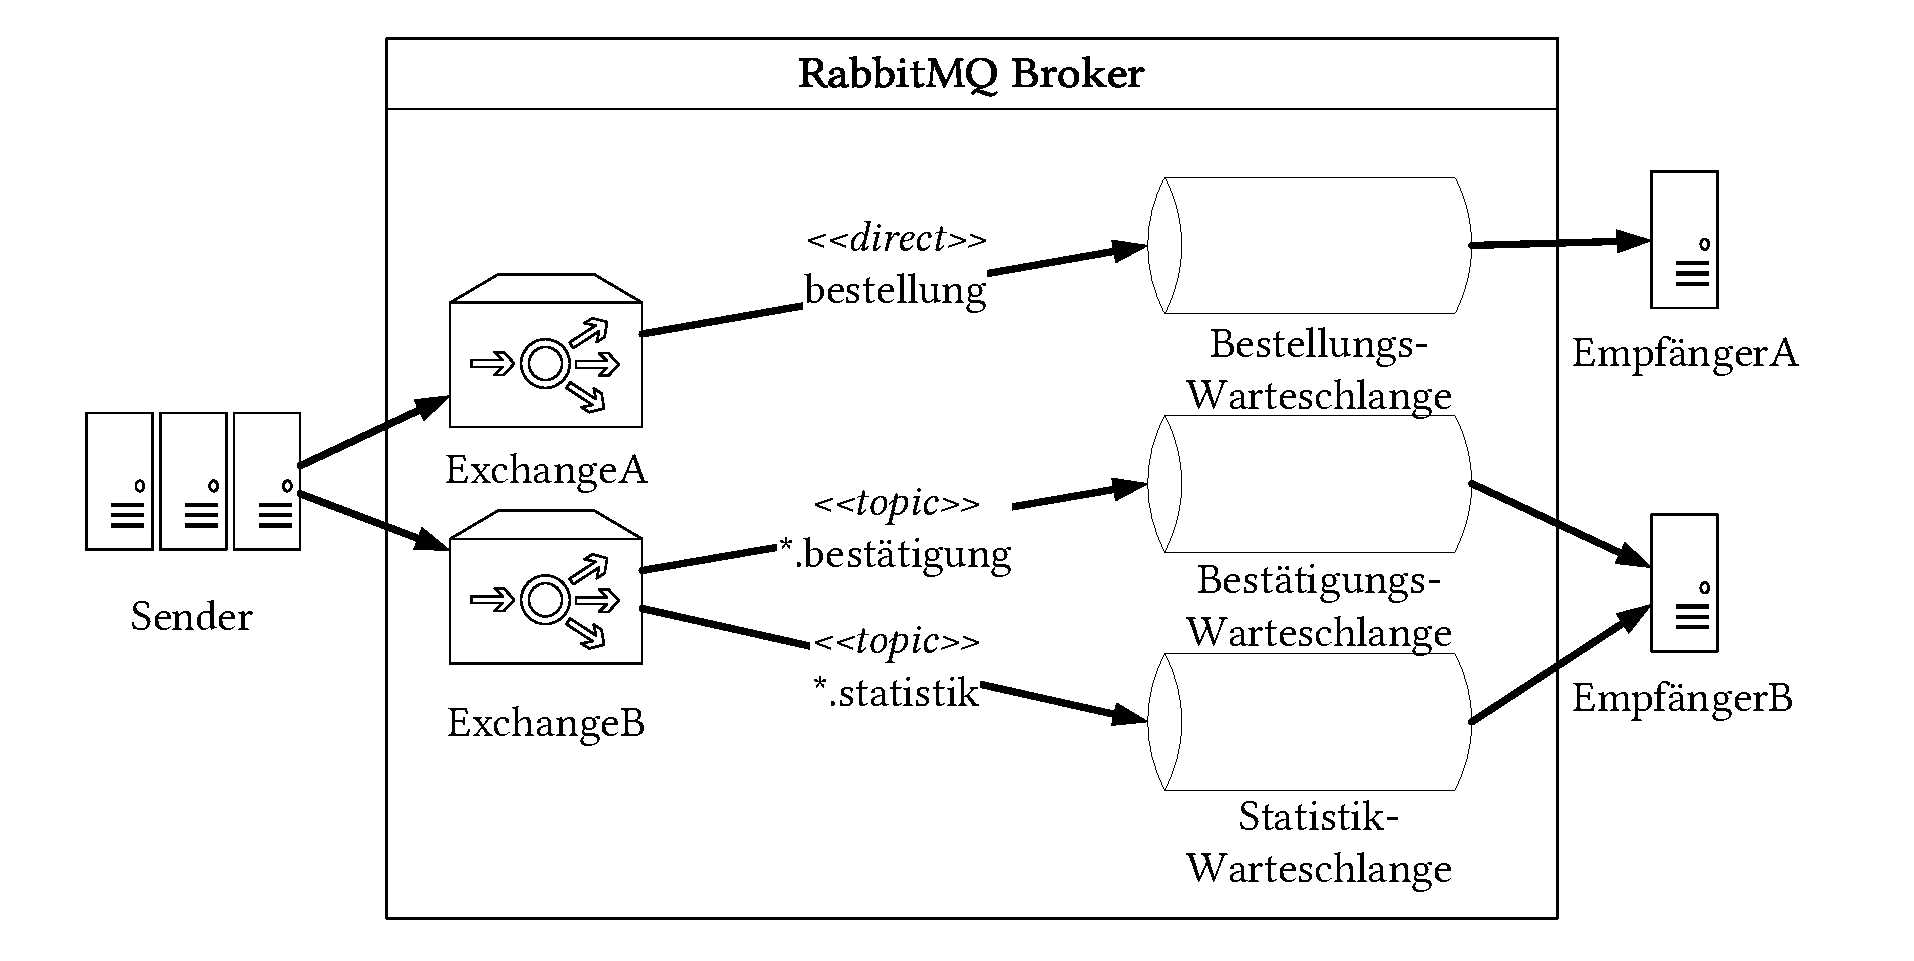
\includegraphics[width=1\textwidth]{images/measurement/rmqexample.pdf}
  \caption{Beispiel einer Kommunikation in RMQ}
  \label{img:rmq_architecture}
\end{figure}
%https://www.cloudamqp.com/blog/2015-05-18-part1-rabbitmq-for-beginners-what-is-rabbitmq.html

%https://www.cloudamqp.com/blog/2018-01-08-part2-rabbitmq-best-practice-for-high-performance.html
Da in dieser Arbeit der Fokus auf der Performance einer MOM liegt, wurden Anhand von Literatur untersucht, für welche der beschriebenen Interaktionstypen RMQ eine hohe Performance erreichen kann. Dazu konnten in (Rmqbuch) die folgenden Eigenschaften und Konfigurationsmöglichkeiten identifiziert werden. RMQ funktioniert am besten, wenn der Füllstand einer Warteschlange klein gehalten wird. Ein Nachricht die in eine leere Warteschlange abgelegt wird, geht direkt an einen Empfänger. Je mehr Nachrichten sich in der Warteschlange befinden, desto länger dauert es diese zu bearbeiten. Wenn der Durchsatz eine wichtige Rolle spielt und die Warteschlangen nicht voll laufen sollen, ist das Setzen einer maximalen Länge der Warteschlange oder das Setzen der Lebensdauer für Nachrichten empfohlen. Dabei bleibt die Warteschlange kurz und neue Nachrichten werden vom Kopf der Warteschlange verworfen, falls sie länger als festgelegt wird. Einen weiteren Performance-Einfluss haben Lazy-Warteschlangen. Dabei werden die Nachrichten einer Warteschlange direkt auf die Festplatte, anstatt in den Hauptspeicher, geschrieben. Das Ziel dabei ist, sehr lange Warteschlangen unterstützen zu können. Dies kann aus verschiedenen Gründen nötig sein:
\begin{itemize}
    \item Empfänger können aus verschiedenen Gründen ausfallen
    \item Plötzlicher anstieg ankommender Nachrichten
    \item Empfänger sind langsamer als normal
\end{itemize}
Das bedeutet, dass Hauptziel von Lazy-Warteschlangen vor allem eine hohe Zuverlässigkeit ist. Da aber die Festplatte anstatt der Hauptspeicher verwendet wird um die Nachrichten zu verwalten, ist diese Konfiguration langsamer. Im Fall dass Performance bevorzugt wird, sollte also auf Lazy-Warteschlangen verzichtet werden. Der Unterschied von Lazy-Warteschlangen zu persistenen Nachrichten, die auch auf die Festplatte geschrieben werden, ist das bei persistenen Nachrichten der Sender entscheidet, ob die Nachricht persistiert wird. Bei Lazy-Warteschlangen, legt der Besitzer der Warteschlange fest, welche Nachrichten persisitiert werden. Der Durchsatz von RMQ kann außerdem dadurch erhöht werden, dass mehrere Warteschlangen verwendet werden. Zum Einen kann eine einzelne Warteschlange nicht mehr als ca. 50\,000 Nachrichten bearbeiten. Zum anderen sind Warteschlangen einfädig. Das heißt, dass der beste Durchsatz auf einem System möglich ist, bei dem es genau so viele Warteschlangen wie Kerne hat. 

In der Folgenden Ausmessung von RMQ wurden diese und weitere Konfiguration untersucht um zu prüfen ob sie einen messbaren Einfluss auf die Performance haben.

\section{Benchmark}
Im Folgenden soll RMQ ausgemessen werden um quantitative Daten ableiten zu können. Dazu werden in \autoref{sec:testmachine} zunächst die Testmaschinen vorgestellt, mit denen die Messungen durchgeführt wurden. Im Anschluss werden in \autoref{sec:rmqBenchmark} die Ergebnisse der einzelnen Messungen vorgestellt und in \autoref{sec:rmqZusammenfassung} zusammengefasst.

\subsection{Testmaschinen}
\label{sec:testmachine}
Die Ausmessung mit zwei virtuellen Servern ausgeführt, die von bwCloud \footnote{https://www.bw-cloud.org/} zur Verfügung gestellt wurden. Die Systemspezifikation der beiden Server ist in \autoref{tab:systespec} aufgelistet. Beide Systeme haben die gleiche Systemspezifikation und haben RMQ Version 3.7.8 installiert. Für die Ausmessung wurden zwei Szenarien betrachtet. Der Aufbau dieser ist in \autoref{img:machineoverview} abgebildet. In \autoref{img:machineoverview}a ist der Fall zu sehen, bei dem sich Sender, Empfänger und der RMQ Broker auf der selben Maschine befinden. Damit soll RMQ unter den bestmöglichen Umständen ausgemessen werden. Im Folgenden wird dieses Szenario als \textit{lokal} bezeichnet. Das andere Szenario ist in \autoref{img:machineoverview}b zu sehen. Dabei befindet sich der RMQ-Broker auf der einen Maschine und Sender und Empfänger auf der anderen. Damit sollen Netzwerkeffekte ausgemessen werden. Im Folgenden wird dieses Szenario als \textit{remote} bezeichnet. Die Netzwerklatenz zwischen beiden Systemen wurde durch eine zweiminütige Messung ermittelt. Die durchschnittliche Netzwerklatenz beträgt dabei 0,556 ms. 

\begin{table}
  \centering
  \begin{tabular}{|l|l|l|l|l|}
    Hauptspeicher & Festplatte & Anzahl vCPUs & GHz & Betriebssystem \\
    \hline
     4 GB & 15 GB & 2 & 2.4 GHz & Ubuntu 18.04
  \end{tabular}
	\caption{\label{tab:systespec} bwCloud VM Spezifikation}
\end{table}

\begin{figure}
\center
  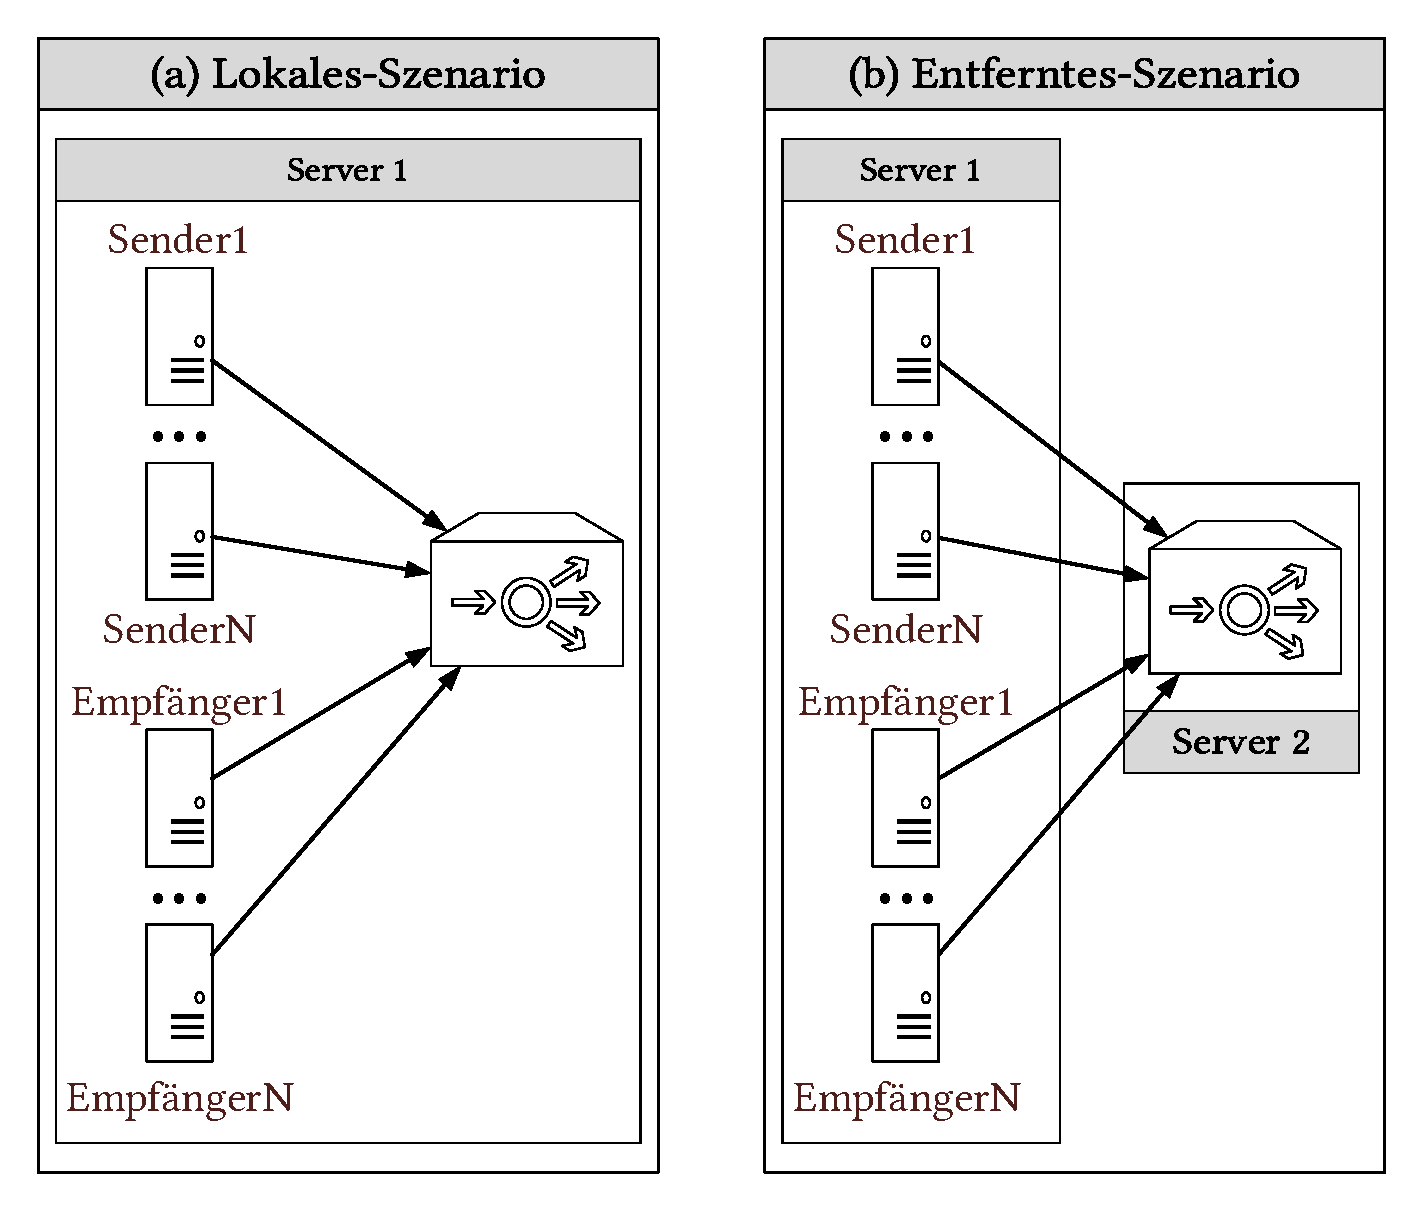
\includegraphics[width=1\textwidth]{images/measurement/benchmarkSzenarioOverview.pdf}
  \caption{Die Beiden Testszenarien}
  \label{img:machineoverview}
\end{figure}

\subsection{Ausmessung von RMQ}
\label{sec:rmqBenchmark}
Im Folgenden wird beschrieben, wie RMQ ausgemessen wurde, um mit den Ergebnissen die Modelle kalibrieren zu können. Um RMQ auszumessen wurde das Performance-Werkzeug von RMQ benutzt\footnote{https://github.com/rabbitmq/rabbitmq-perf-test}. Dieses erlaubt es, die gesendeten und empfangenen Nachrichten und ihre Latenz zu messen. Die Latenz ist hierbei als die Zeit definiert, die eine Nachricht braucht bis sie vom Empfänger aus der Warteschlange entnommen wird, nachdem sie vom Sender dort abgelegt wurde. Das Werkzeug kann konfiguriert werden um bestimmte Szenarien zu simulieren. Unter anderem lässt sich die Anzahl der zu sendenden und zu empfangenen Nachrichten pro Sekunde einstellen. Weitere Konfigurationsmöglichkeiten sind Nachrichtengröße und die Anzahl der Sender und Empfänger. Im Folgenden sollen die Ergebnisse der Messungen vorgestellt werden. Dabei werden die einzelnen Ergebnisse und ihr Versuchsaufbau vorgestellt. Jedes Ergebnis wird wie folgt beschrieben: 
\begin{itemize}
    \item Vorstellung des Szenarios
    \item Beobachtungen des Systemverhaltens
    \item Messergebnisse
\end{itemize}
Jede Messung wurde zehn mal durchgeführt. Die einzelnen Konfiguration wurde jeweils zwei Minuten ausgeführt. 



\subsubsection{Latenz einer nicht-persistenter Nachricht}
\label{sec:oneMsgLatency}
Zunächst soll geprüft werden wie groß die Latenz einer einzelnen, nicht persistenten, Nachricht ist. Dabei wurde auch die Größe einer Nachricht betrachtet. Dazu wurde die Senderate auf eine Nachricht pro Sekunde reduziert und die Nachrichtengröße zwischen 1 KByte und 1 MByte variiert. Für diese Messung wurde das \textit{lokal}-Szenario verwendet. Erwartet wird, dass die Latenz einer Nachricht mit ihrer Nachrichtengröße steigt.
%B
Die Ergebnisse sind in \autoref{img:senderate1-A} abgebildet. Neben den Messergebnissen ist eine Linie durch die Mediane der einzelnen Messungen gezogen. Dabei ist zu sehen, dass die Latenz einer Nachricht mit Ansteigen der Nachrichtengröße auch ansteigt. Somit verhält sich das System wie erwartet.
\begin{figure}
\center
  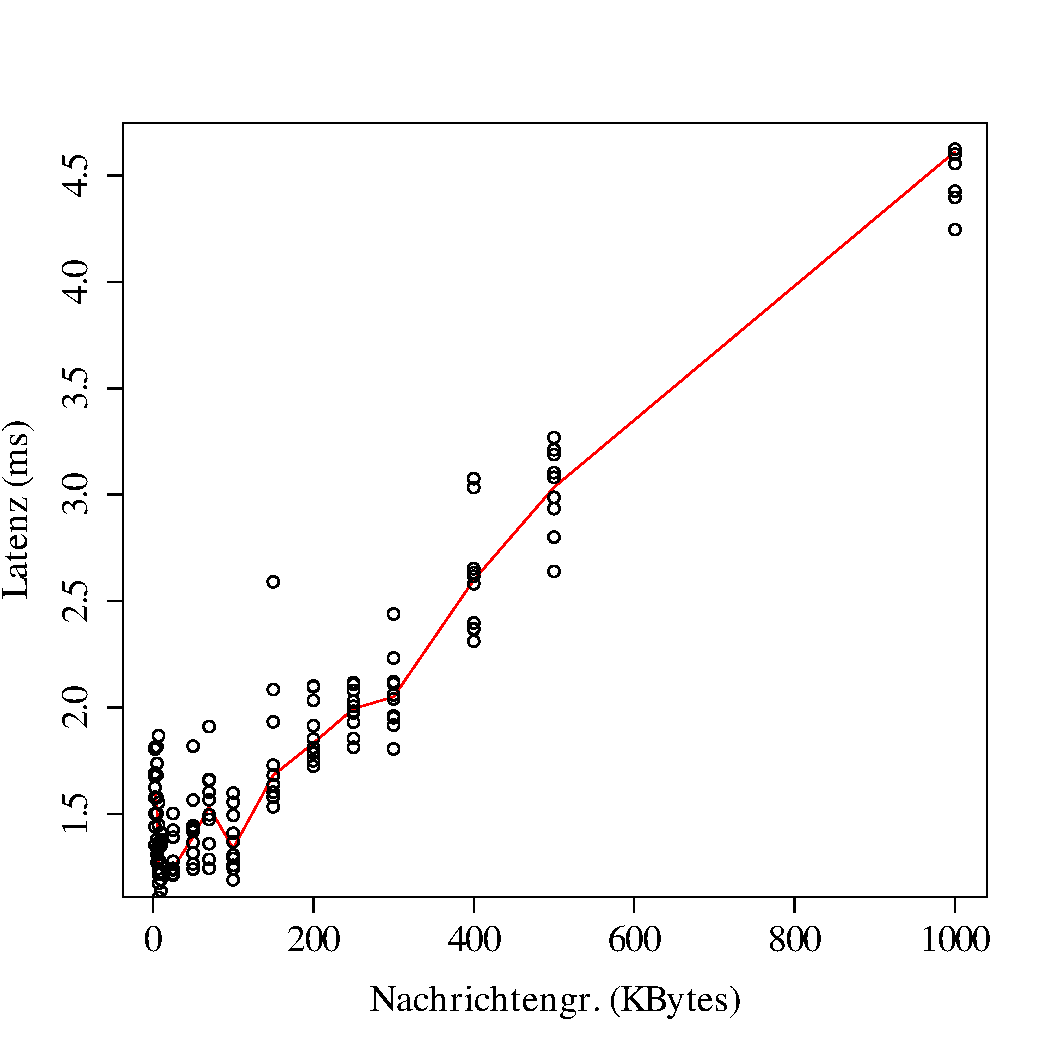
\includegraphics[width=0.7\textwidth]{images/measurement/rate-limit-1-A.pdf}
  \caption{Latenz einer Nachricht im \textit{lokal}-Szenario}
  \label{img:senderate1-A}
\end{figure}

Als nächstes wurde die Latenz einer Nachricht zu einem entfernten RMQ-Broker gemessen. Dazu wurde das \textit{remote}-Szenario verwendet. Die Nachrichtengröße variiert zwischen 1 KByte und 1 MByte. Erwartet wird, dass zu der bereits gemessenen Latenz einer Nachricht die Netzwerklatenz dazugerechnet wird.

%B
Die Ergebnisse sind in \autoref{img:senderate1-B} zu sehen. Dabei ist durch die Mediane der einzelnen Messergebnisse eine Linie gezogen. Zu sehen ist, dass auch hier die Latenz mit Ansteigen der Nachrichtengröße wächst. Die Differenz, zur vorherigen Messung, entspricht der gemessenen Netzwerklatenz.
%E
Somit ist neben der Nachrichtengröße auch die Netzwerklatenz ein Faktor, der die Latenz einer Nachricht beeinflusst.

\begin{figure}
\center
  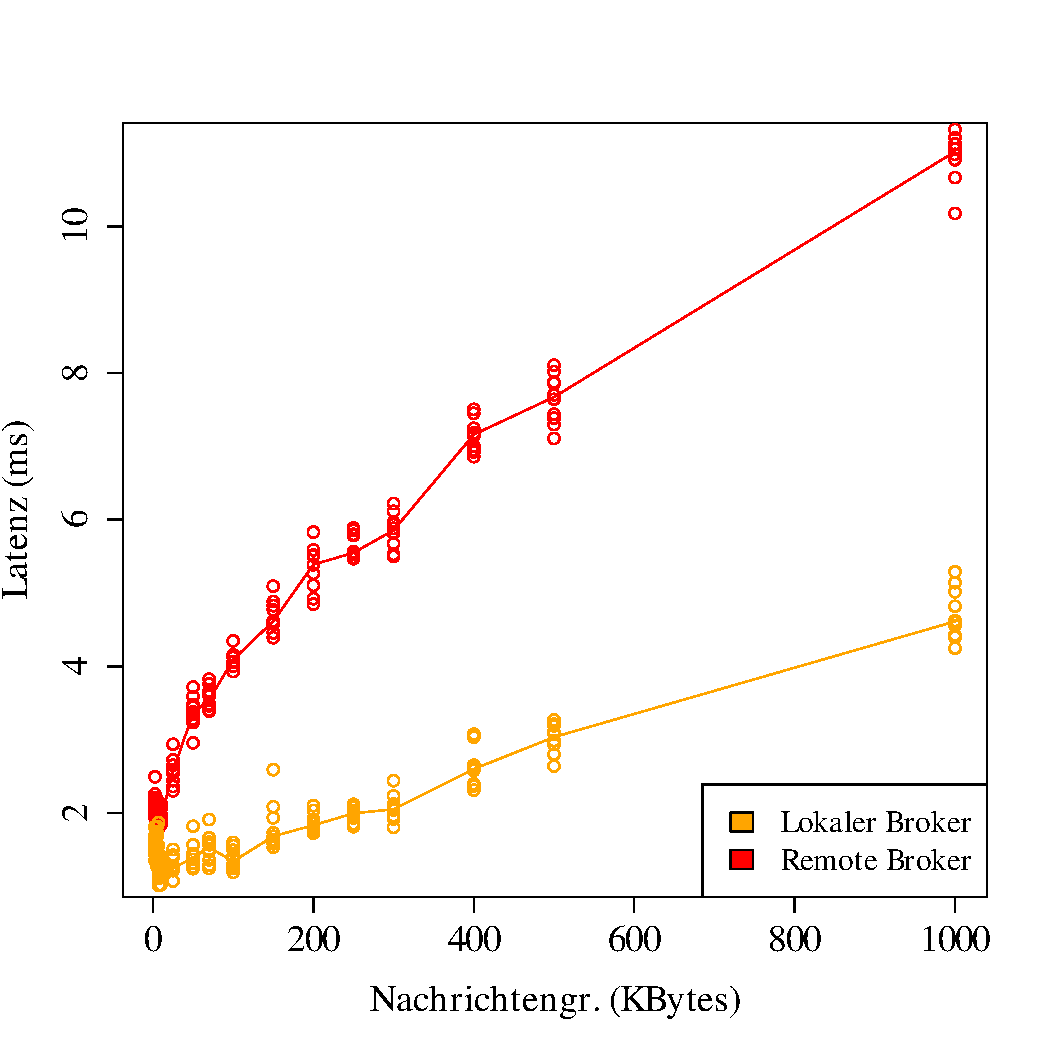
\includegraphics[width=0.7\textwidth]{images/measurement/rate-limit-1-AvsB.pdf}
  \caption{Latenz einer Nachricht im \textit{remote}-Szenario}
  \label{img:senderate1-B}
\end{figure}

\subsubsection{Latenz einer persistente Nachricht}
Da zuvor die Latenz nicht-persistenter Nachrichten ausgemessen wurde, wird in dieser Messung die Latenz einer persistenten Nachricht ausgemessen. Die Senderate wurde auf eine Nachricht pro Sekunde reduziert und die Nachrichtengröße zwischen 1 KByte und 1 MByte variiert. Für diese Messung wurde das \textit{lokal}-Szenario verwendet. Erwartet wird, dass die Latenz einer persistenten Nachricht größer als die einer nicht-persistenten Nachricht ist, da die Nachricht auch auf die Festplatte geschrieben wird.
%B
In \autoref{img:senderatepersisten} sind die Ergebnisse der Messung zu sehen. Außerdem wurde zu Vergleich auch die nicht-persistente Messung eingezeichnet. Wie erwartet ist die Latenz einer persistenten Nachricht größer. Der Grund hierfür ist, dass die Nachricht auch auf die Festplatte geschrieben wird, um eine Zustellung zu garantieren. Somit hat die Wahl zwischen nicht-persistenten und persistenten Nachrichten einen Einfluss auf die Performance.

\begin{figure}
\center
  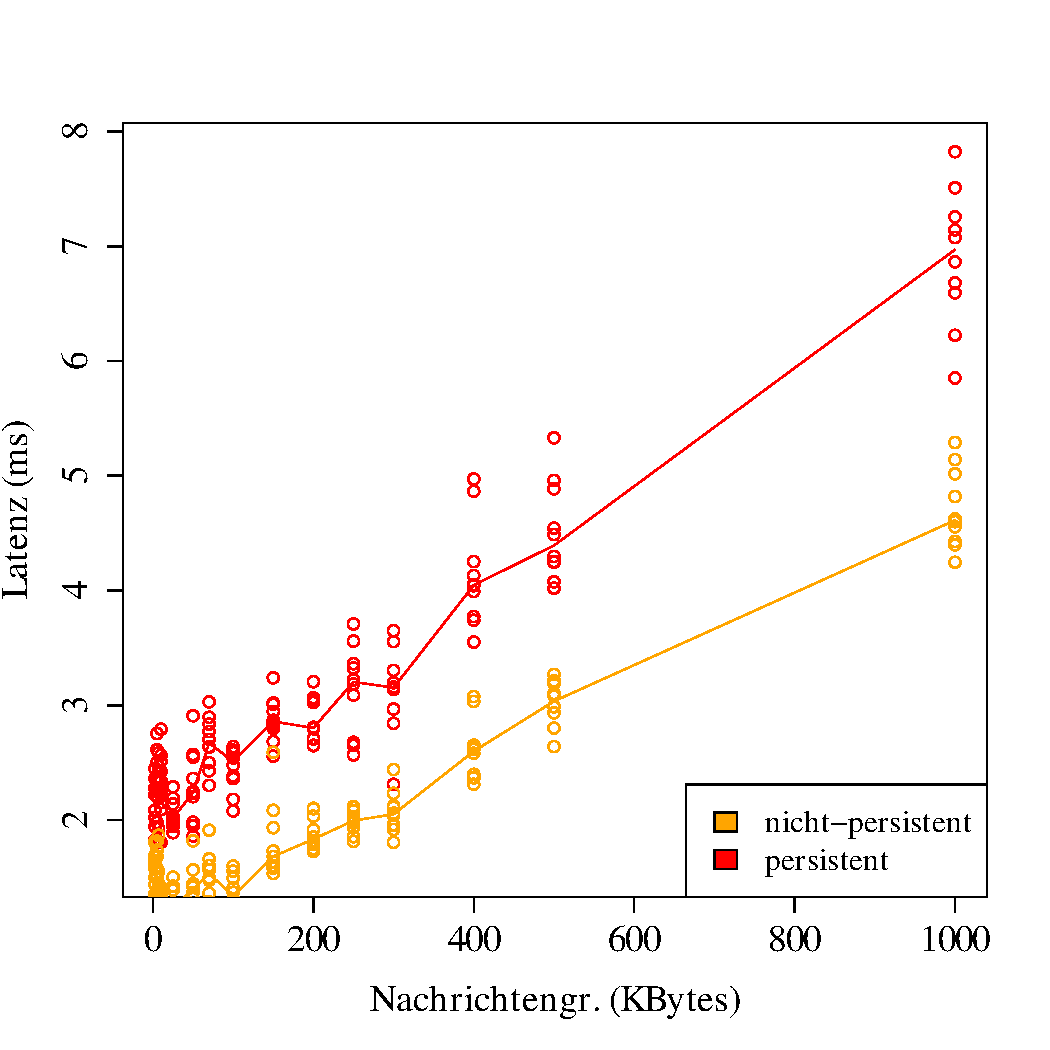
\includegraphics[width=0.7\textwidth]{images/measurement/persistentVsNonPersistent.pdf}
  \caption{Latenz einer nicht-persistenten im Vergleich zu einer persistenten Nachricht.}
  \label{img:senderatepersisten}
\end{figure}
\subsubsection{Nachrichtengröße}
Da in den vorherigen Messung die Nachrichtengröße als Einflussfaktor auf die Latenz und somit die Performance identifiziert wurde, sollen im Folgenden weitere Effekte im Zusammenhang mit der Nachrichtengröße untersucht werden. Dazu wurde ein Sender und ein Empfänger eingerichtet. Beide senden und empfangen Nachrichten so schnell sie können; die oben beschriebene Limitierung der Senderate auf eine Nachricht pro Sekunde ist somit aufgehoben. Die Nachrichtengröße variiert zwischen 1 KByte und 200 KByte. Es wurde mit dem \textit{lokal}-Szenario ausgemessen. Erwartet wird, dass sich mit zunehmender Nachrichtengröße die insgesamt pro Sekunde gesendete Nachrichtenmenge verringert. Gleichzeitig sollte die insgesamt gesendete Datenmenge zunehmen, da die Nachrichten weniger Routing-Overhead beim RMQ-Broker verursachen.
%B
In \autoref{img:msgsize} sind die Ergebnisse dieser Messung abgebildet. Durch die jeweiligen Mediane wurde eine Linie gezogen. Die Auswirkung der Nachrichtengröße auf die Senderate ist dabei in \autoref{img:msgsize}a zu sehen. Diese nimmt, wie erwartet, mit zunehmender Größe ab. In \autoref{img:msgsize}b ist die insgesamt gesendete Datenmenge zu sehen. Auch hier verhält sich das System wie erwartet und die insgesamt gesendete Datenmenge nimmt zu.
\begin{figure}
\center
  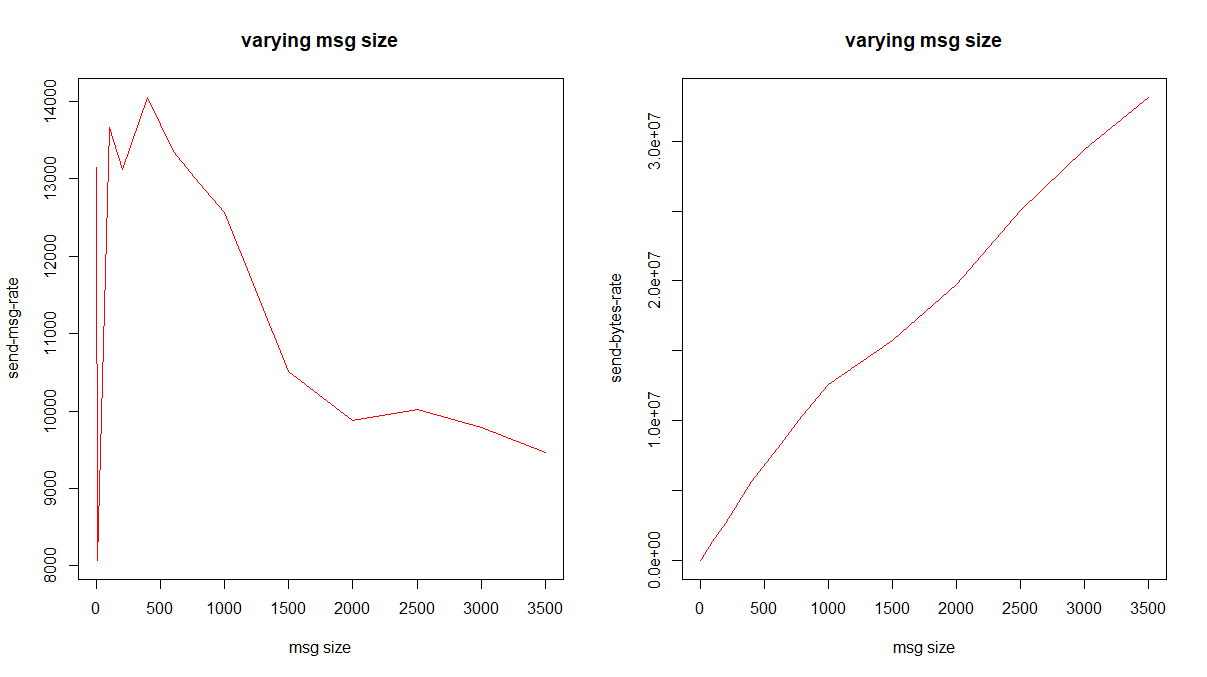
\includegraphics[width=0.7\textwidth]{images/msg-size.png}
  \caption{TODO besseres Bild}
  \label{img:msgsize}
\end{figure}
%E
Wie bereits erwähnt lässt sich dieser Effekt darauf zurückführen, dass bei größeren Nachrichten der Broker weniger Routing-Overhead hat, als bei kleineren.
%https://www.rabbitmq.com/blog/2012/04/25/rabbitmq-performance-measurements-part-2/

\subsubsection{Maximale zu sendende Datenmenge}
\label{sec:maxthroughput}
Nachdem die Effekte der zunehmende Nachrichtengröße geprüft wurden, soll nun geprüft werden wie groß die insgesamt mögliche Datenmenge ist, die gesendet und empfangen werden kann. Dazu wurden Nachrichten der Größe 1 KByte bis 200 KByte gesendet. Es wurden zwei Messungen durchgeführt. Im Fall der ersten Messung existiert ein Sender und kein Empfänger, bei der zweiten Messung ein Sender und ein Empfänger. Die Messung wurde mit dem \textit{lokal}-Szenario durchgeführt. Erwartet wurde, dass die Messung ohne Empfänger einen höheren Durchsatz ermöglicht, da diese direkt verworfen werden. 
%B
Die Ergebnisse sind in \autoref{img:maxByteThroughputA} zu sehen. Die Abbildung zeigt, dass wenn kein Empfänger vorhanden ist, mit zunehmender Nachrichtengröße die insgesamt gesendete Datenmenge an einen Wert bei ca. 1.5 GByte pro Sekunde annähert. Wenn ein Empfänger vorhanden ist, nähert sich die Datenmenge an 700 MByte pro Sekunde an. Dieser Uterschied lässt sich auf den fehlenden Empfänger bzw. die fehlende Warteschlange zurückführen. Es gibt somit keinen Schreib-Overhead, da die Nachricht weder im Speicher, noch auf der Festplatte abgelegt wird.
\begin{figure}
\center
  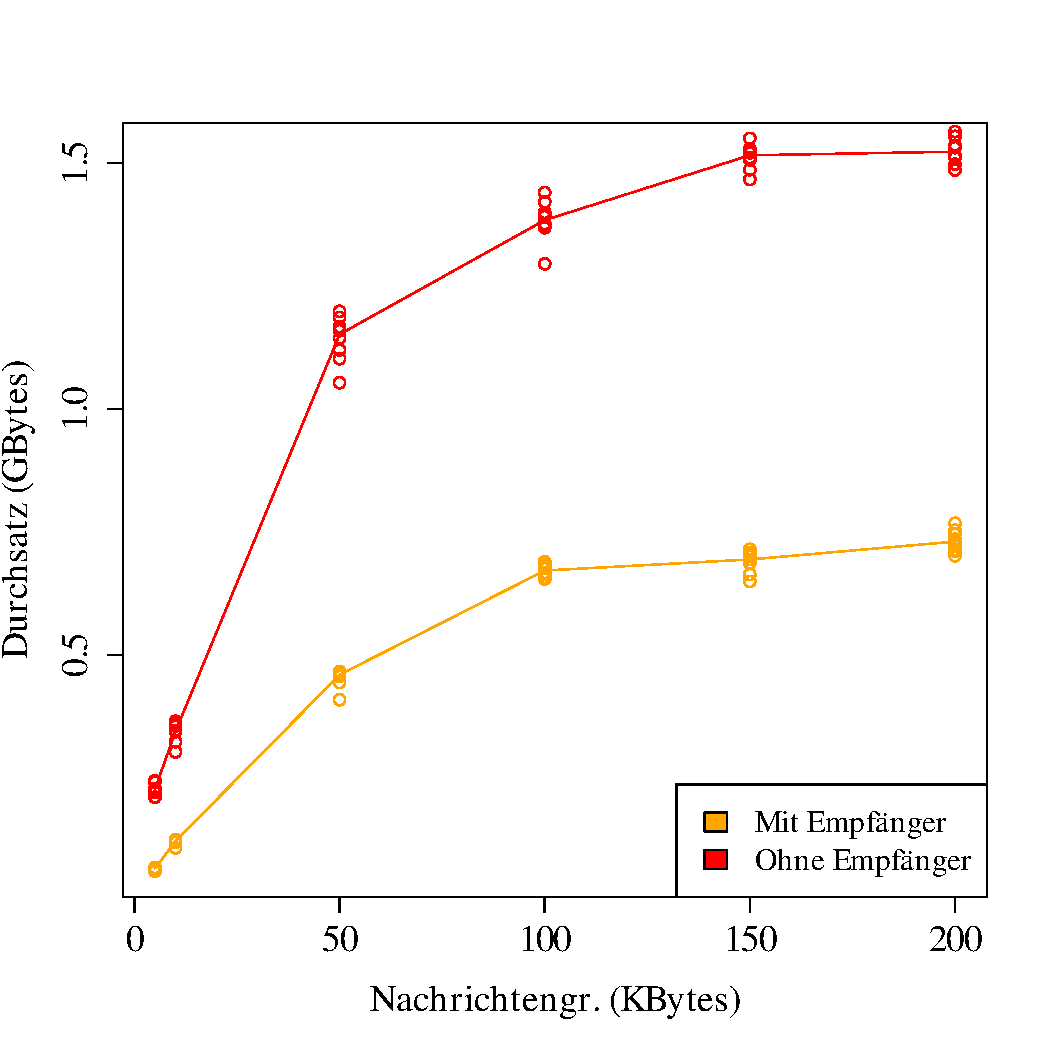
\includegraphics[width=0.7\textwidth]{images/measurement/rate-limit-unlimited-consumer-vs-no-consumer.pdf}
  \caption{Maximale Datenmenge im \textit{lokal}-Szenario}
  \label{img:maxByteThroughputA}
\end{figure}

%Ein weiterer Effekt ist in \autoref{img:unlimitedLatency} zu sehen. Dabei ist zu sehen, dass die Latenz sinkt wenn mehr Nachrichten auf einmal gesendet werden.
%\begin{figure}
%\center
%  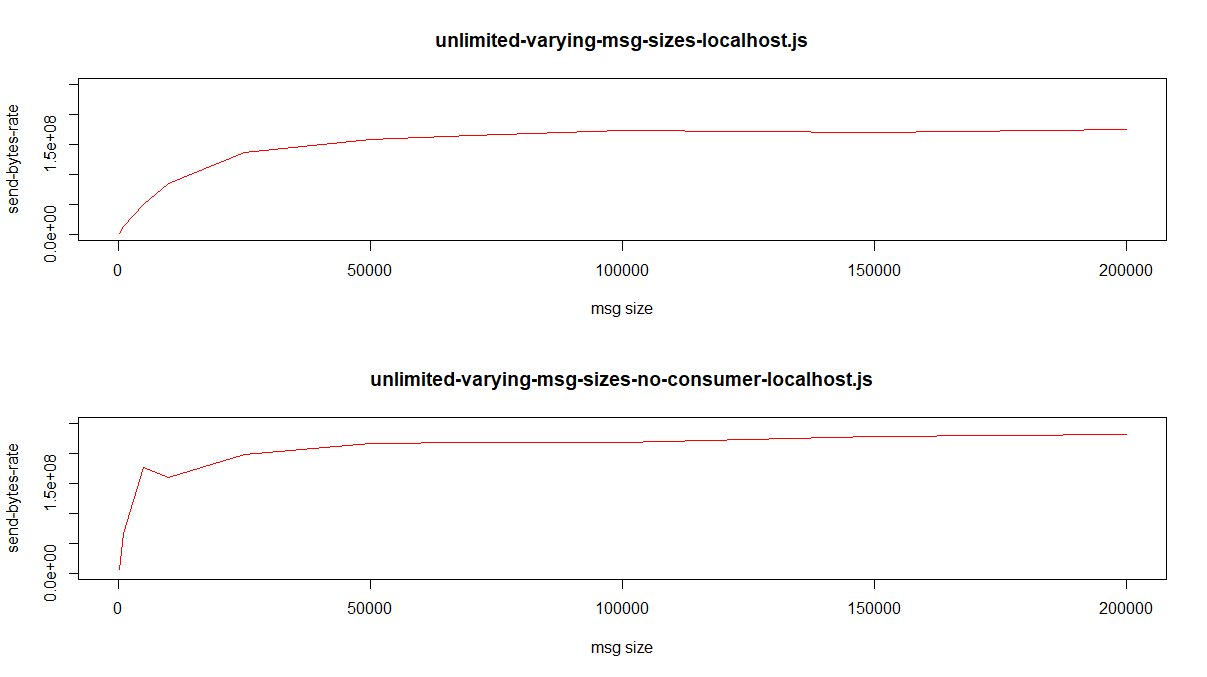
\includegraphics[width=1\textwidth]{images/max-byte-throughput-A.pdf}
%  \caption{Max Datenmenge, Latenz, Testsystem A}
%  \label{img:unlimitedLatency}
%\end{figure}
%Dieser Effekt laesst sich darauf zurueckfuehren, dass wenn mehrere Nachrichten auf einmal gesendet werden der Broker weniger routing overhead hat.

Die selbe Messung wurde mit dem \textit{remote}-Szenario durchgeführt. Erwartet wird, dass die Datenmenge kleiner ist, da die Netzwerkverbindung beachtet werden muss. 
%B
Die Gegenüberstellung für den Fall, dass es einen Sender, aber keine Empfänger gibt ist in \autoref{img:maxByteThroughputNoConsumerB} zu sehen. Die an das \textit{remote}-System gesendete Datenmenge ist dabei deutlich kleiner als zuvor. Diese nähert sich dem Wert von ca. 700 Mbyte anstatt 1.5 Gbyte an. Die Messung mit Empfänger ist in \autoref{img:maxByteThroughputB} abgebildet. Auch hier ist die gesendete Datenmenge deutlich kleiner und nähert sich nur einem Wert von ca. 400 Mbyte anstatt 700 Mbyte an.
\begin{figure}
\center
 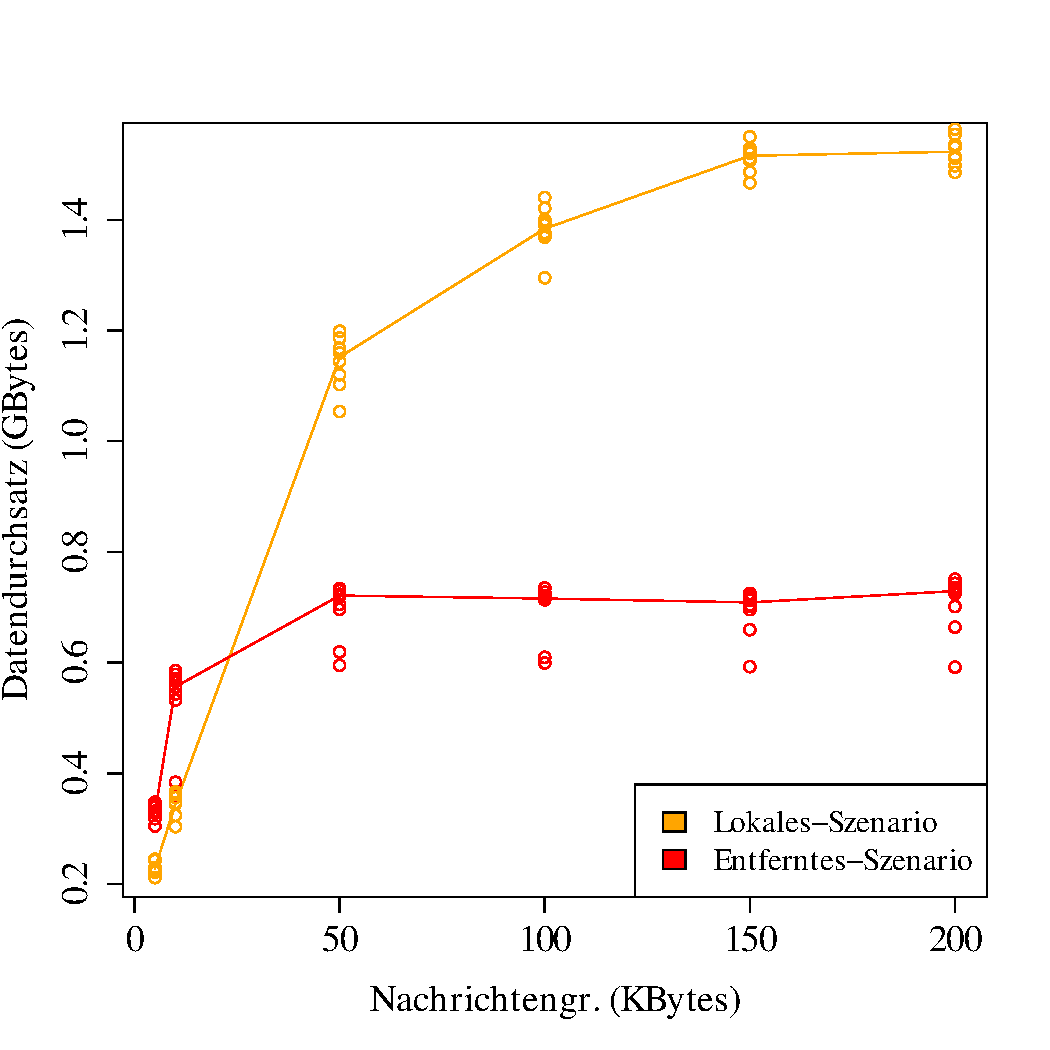
\includegraphics[width=0.7\textwidth]{images/measurement/rate-limit-unlimited-no-consumer-AvsB.pdf}
  \caption{Maximale Datenmenge ohne Empfänger im \textit{remote}-Szenario}
  \label{img:maxByteThroughputNoConsumerB}
\end{figure}
\begin{figure}
\center
 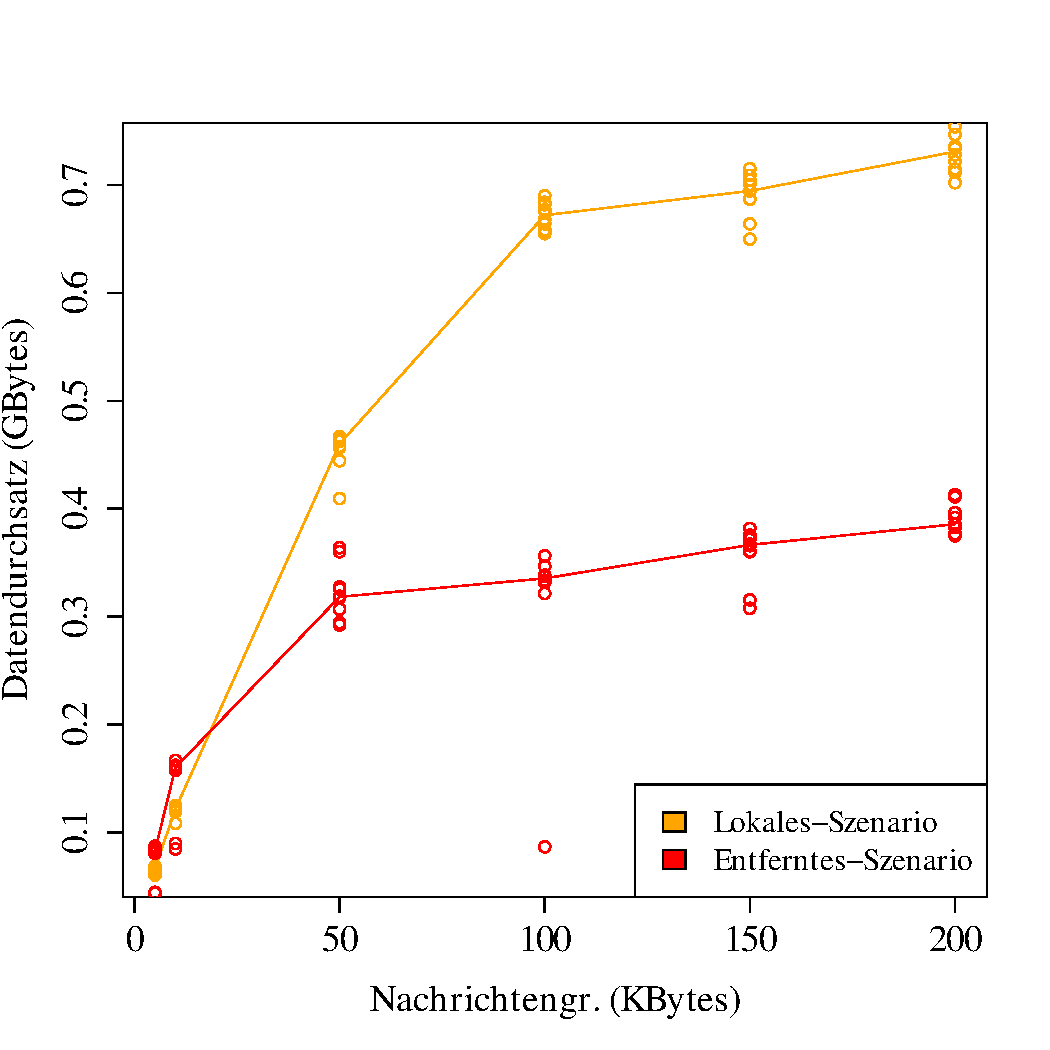
\includegraphics[width=0.7\textwidth]{images/measurement/rate-limit-unlimited-AvsB.pdf}
  \caption{Maximale Datenmenge mit Empfänger im \textit{remote}-Szenario}
  \label{img:maxByteThroughputB}
\end{figure}
%E
Obwohl beide Testmaschinen vom selben Anbieter sind, unterscheiden sich die möglichen Datenmengen zwischen einem lokalen und entfernten Broker. Dieser Unterschied kann auf den möglichen Durchsatz einer Netzwerkverbindung zuruckgeführt werden. Somit ist der mögliche Durchsatz einer Verbindung zwischen Sender, Empfänger und dem Broker ein limitierender Faktor und hat somit auch Einfluss auf die Performance des Gesamtsystems.

\subsubsection{Ansteigen des Füllstands der Warteschlange}
\label{sec:queueGrowth}
Diese Messung untersucht die Auswirkung des Warteschlangen-Füllstands auf die Latenz der einzelnen Nachrichten. Die Messung besteht aus einem Sender und einem Empfänger. Die Senderate beträgt zwei Nachrichten pro Sekunde, der Empfänger empfängt jedoch nur eine Nachricht pro Sekunde. Die Nachrichten sind dabei 1 Kbyte groß. Die Messung wurde mit \textit{lokal}-Szenario durchgeführt. Erwartet wird, dass die Latenz der Nachrichten mit Ansteigen des Warteschlangenfüllstandes wächst, da die Nachrichten länger in der Warteschlange warten, bis sie abgeholt werden.
%B
In \autoref{img:queuegrowth} sind die Messergebnisse abgebildet. Dabei ist in \autoref{img:queuegrowth}a der Füllstand der Warteschlange zu sehen. Diese wächst pro Sekunde um eine Nachricht die nicht abgeholt wird an. In \autoref{img:queuegrowth}b ist die Latenz der Nachrichten abgebildet. Wie erwartet steigt diese mit Ansteigen des Füllstandes, da die Nachrichten länger in der Warteschlange warten müssen, bis sie abgeholt werden.
\begin{figure}
\center
  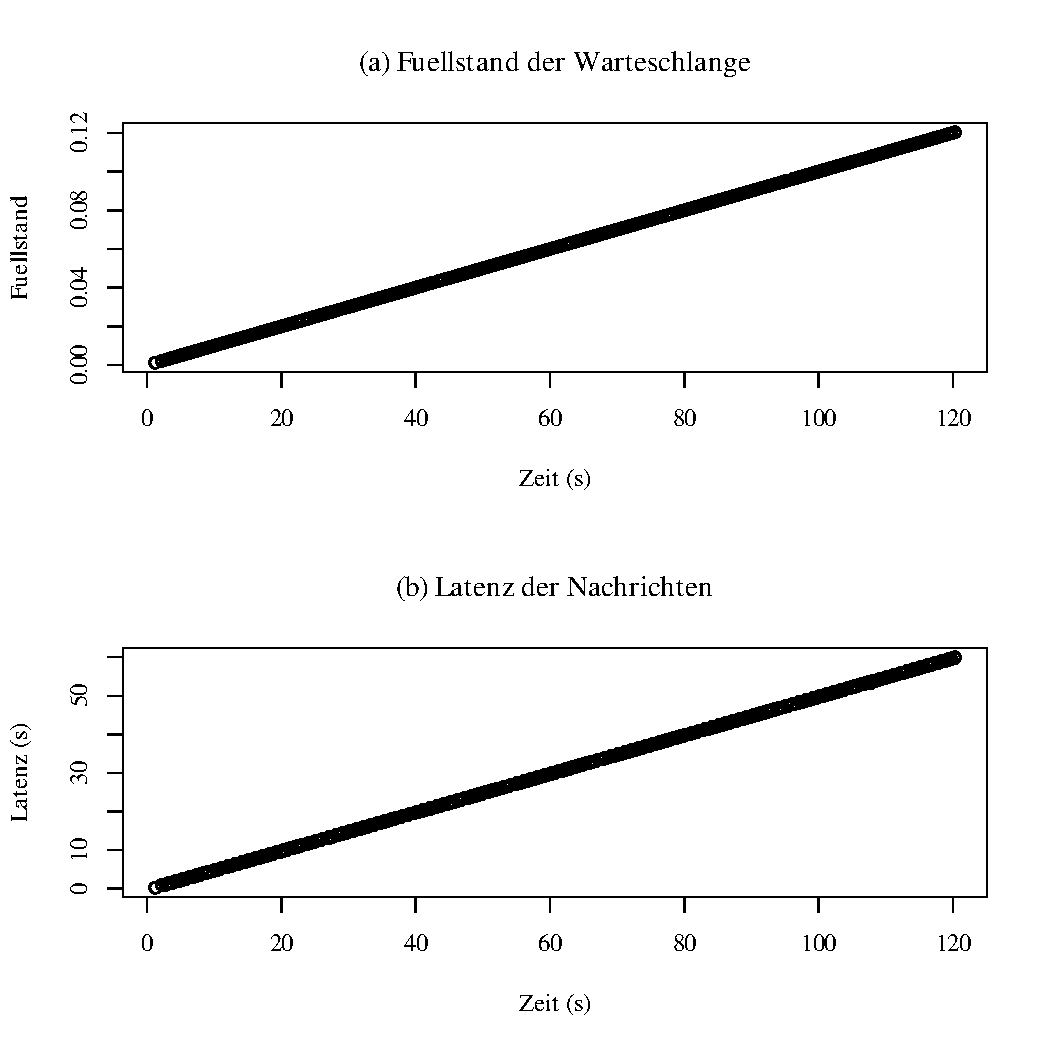
\includegraphics[width=0.7\textwidth]{images/measurement/queuegrowth.pdf}
  \caption{Wachstum einer Warteschlange und Auswirkung auf die Latenz.}
  \label{img:queuegrowth}
\end{figure}

\subsubsection{Konfiguration: Warteschlangenlänge begrenzen}
\label{sec:maxlength}
Die vorherige Messung hat gezeigt, das sich das Anwachsen der Warteschlange negativ auf die Latenz der Nachrichten auswirkt. Wie bereits erwähnt erlaubt RMQ einige Konfigurationen. Eine davon ist das Setzen einer maximal Länge für Warteschlangen. Damit soll die Warteschlange kurz gehalten werden und die Latenz der Nachrichten klein. Damit wird dem Effekt der in der vorherigen Messung untersucht wurde, entgegengewirken. Standardmäßig wird der Kopf der Warteschlange verworfen. Mit der folgenden Messung soll diese Konfiguration untersucht werden. Dazu wurden drei Warteschlange angelegt. Diese hatten eine maximal Länge von 100, 5000 und 50.000 Nachrichten. Die Größe von 50.000 ist die RMQ-Standardgröße für Warteschlangen. Damit man die Auswirkung auf volle Warteschlangen sehen kann wurde die Sende- und Empfangsrate entsprechend angepasst. Die Senderate wurde auf 1000 und die Empfangsrate auf 100 Nachrichten pro Sekunde eingestellt. Die Nachrichten Größe war 100 Bytes. Die Messung wurde mit dem \textit{lokal}-Szenario durchgeführt. Erwartet wird, dass sobald die Warteschlange voll wird, die Latenz nicht mehr zu nimmt. Dieser Moment sollte schneller erreicht werden, je kleiner die Warteschlange ist.
%B
Die Ergebnisse sind in \autoref{img:maxlength} abgebildet. Wie erwartet wachsen die Latenzen der Nachrichten bei den begrenzten Warteschlangen ab einem bestimmten Moment nicht weiter an. Wie in \autoref{img:maxlength}a und \autoref{img:maxlength}b zu sehen ist, tritt dieser Moment für die kürzere Warteschlange früher ein. In \autoref{img:maxlength}c wächst die Latenz immer weiter.
\begin{figure}
\center
  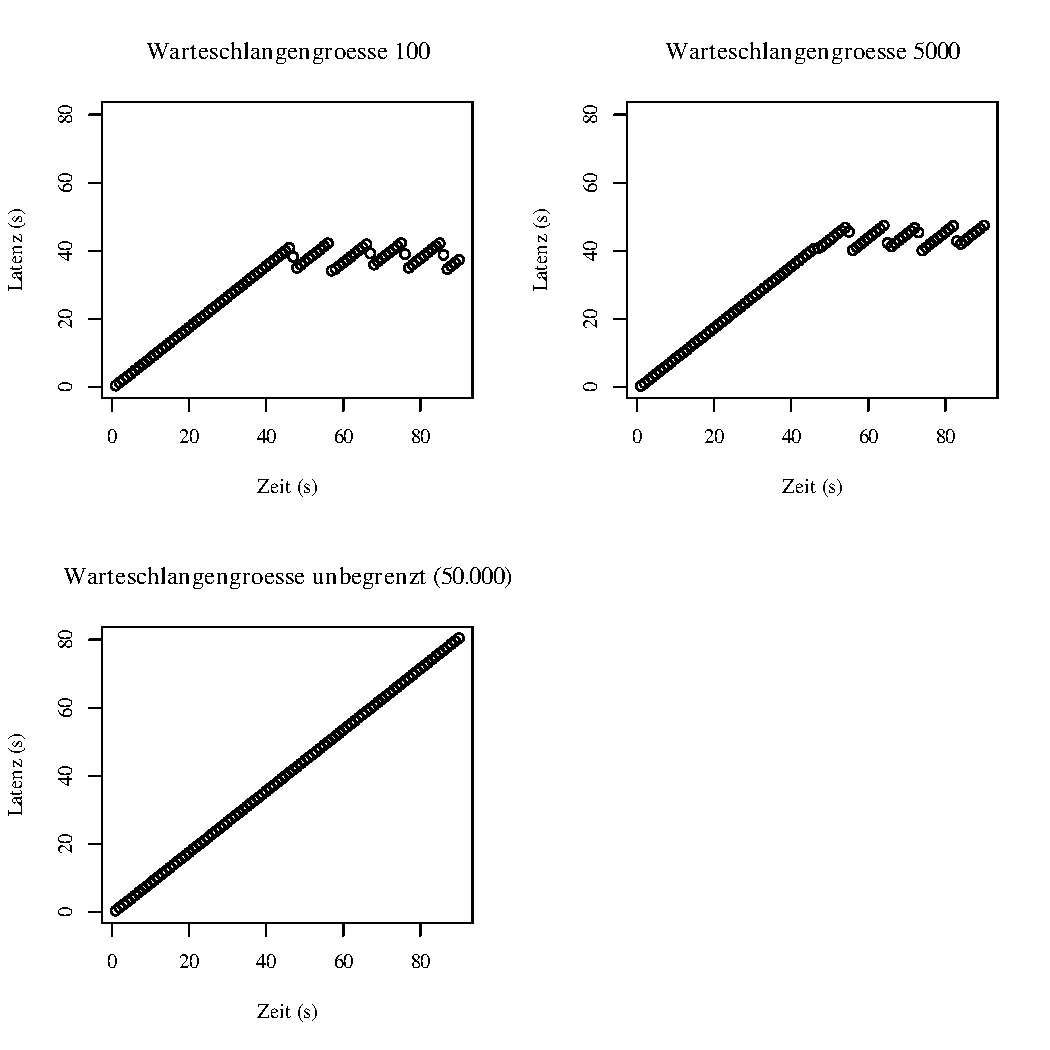
\includegraphics[width=0.7\textwidth]{images/measurement/max-length.pdf}
  \caption{Auswirkung auf die Latenz bei verschieden großen Warteschlangen.}
  \label{img:maxlength}
\end{figure}
%E
Diese Konfiguration zeigt, dass die Warteschlangenbegrenzung einen Einfluss auf die Latenz hat und man diese begrenzen kann, wenn man die Warteschlangengröße begrenzt. Der Nachteil dabei ist, dass Nachrichten verworfen werden, sobald die Warteschlange voll ist. Somit hat auch die Warteschlangengröße einen Einfluss auf die Performance. 

%wenn Queue voll, dann wird Msgrate angepasst

%Flow alarm ab RabbitMQ 2.8.0+ bei Versionen davor verhlaehlt sich RMQ wie in (sec: Speicher ausgeschoepft)

%\subsubsection{Speicher von RMQ ausgeschoepft}
%Nachdem in der Messung davor die Laenge der Warteschlange betrachtet wurde, soll nun untersucht werden ob der Verfuegbare Speicher des Broker einfluss auf die Performanz hat. Dazu wurde auf der Testmaschine B die Hauptspeicher fuer RMQ auf 10 MB gesetzt.  
%Sollte der verfuegbare Speicher des Broker ausgeschoepft sein, wird der MemoryAlarm aktiviert und der Broker blockiert ankommende Nachrichten, bis der Speicher wieder frei ist. Dies ist in (abb) zu sehen.
%TODO beobachtung und Ergebnis



\subsubsection{Konfiguration: Lazy-Warteschlangen}
\label{sec:rmqLazy}
Eine weitere Konfiguration die RMQ ermöglicht sind Lazy-Warteschlangen. Wie bereits erwähnt, werden dabei Nachrichten auf die Festplatte anstatt in den Hauptspeicher geschrieben. In der nächsten Messung soll untersucht werden ob die Konfiguration von Lazy-Warteschlangen Auswirkungen auf die Performance hat. Dabei wurde auch die Größe einer Nachricht betrachtet. Für die Messung wurde die Senderate auf eine Nachricht pro Sekunde reduziert und die Nachrichtengröße zwischen 1 KByte und 1 MByte variiert. Für diese Messung wurde das \textit{lokal}-Szenario verwendet. Erwartet wird, dass die Latenz einer Nachricht, im Vergleich zu nicht-persistenten Nachrichten größer ist. Außerdem sollte die Messung ähnliche Ergebnisse liefern wie die Messung mit persistenten Nachrichten.
%B
In \autoref{img:lazy} ist ein Vergleich der Messung mit nicht-persistenten und den Messergebnissen mit Lazy-Warteschlangen abgebildet. Zu sehen ist, dass die Latenz mit Lazy-Warteschlangen größer ist, als die der nicht-persistenten Nachrichten. Außerdem sind die Messergebnisse dieser Messung und der Messung mit persistenten Nachrichten ähnlich.
\begin{figure}
\center
  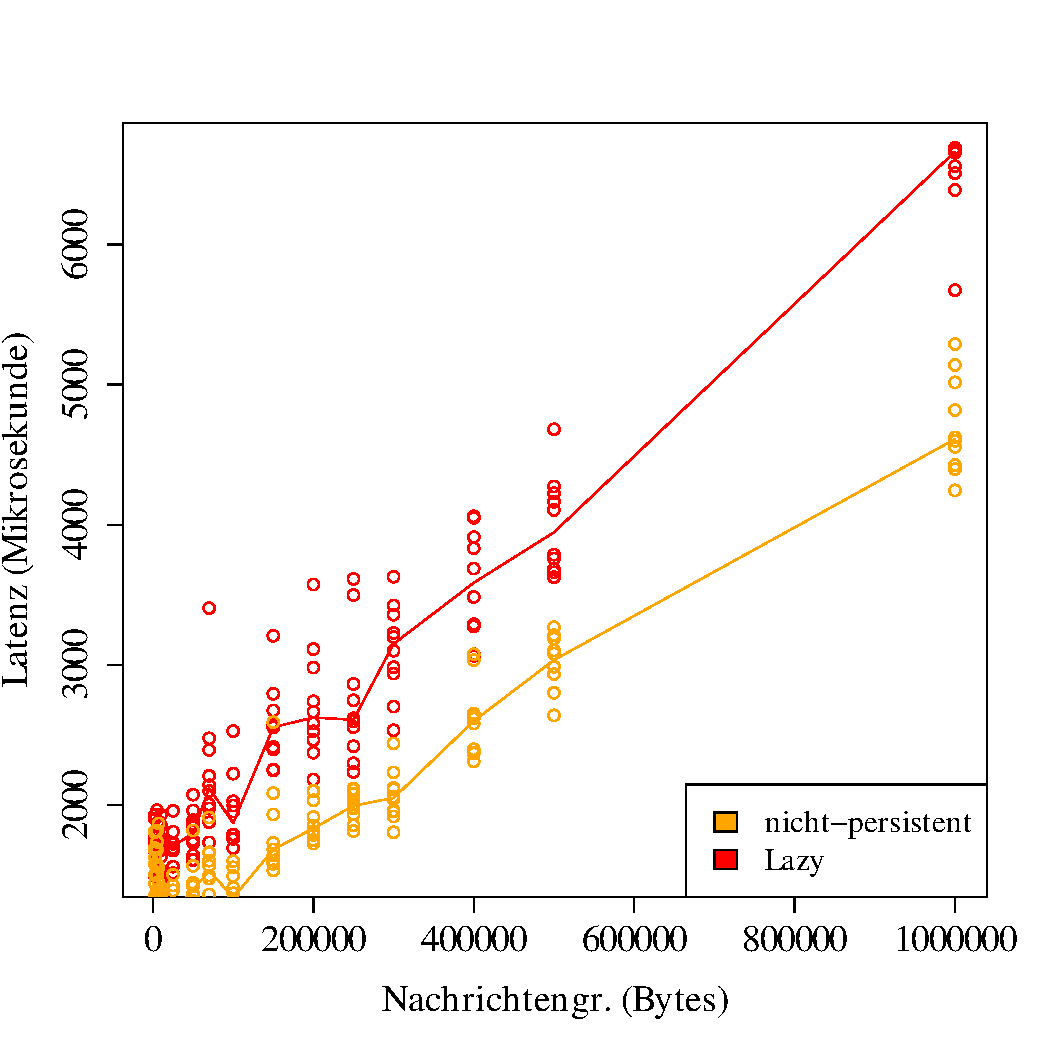
\includegraphics[width=0.7\textwidth]{images/measurement/lazy-queues.pdf}
  \caption{Lazy-Warteschlange im Vergleich mit nicht-persistenten Nachrichten.}
  \label{img:lazy}
\end{figure}
%E
Grund hierfür ist das die Nachrichten auf die Festplatte anstatt in den Hauptspeicher geschrieben werden. Somit hat diese Konfiguration einen ähnlichen Einfluss auf die Performance, wie der Einsatz persistenter Nachrichten.



\subsubsection{Mehrere Empfänger}
\label{sec:varyingConsumer}
In \autoref{sec:queueGrowth} und \autoref{sec:maxlength} war bereits zu sehen, dass volle Warteschlangen einen Einfluss auf die Latenz haben. In dieser Messung soll geprüft werden, ob es einen Unterschied macht einen oder mehrere Empfänger eine Warteschlange abarbeiten zu lassen. Dazu wurde die Senderate eines Senders auf 1000 Nachrichten und die Empfangsrate auf 200 Nachrichten pro Sekunde limitiert. Alle Empfänger greifen auf die selbe Warteschlange zu. Außerdem wurde eine Referenzmessung mit einem Sender und einem Empfänger mit einer Sende- und Empfangsrate von 1000 durchgeführt. Die Messung wurde mit dem \textit{lokal}-Szenario durchgeführt. Erwartet wird, dass es keinen unterschied macht ob ein oder mehrere Empfänger eine Warteschlange abarbeiten.
%B
In \autoref{img:varyingConsumer} sind die Ergebnisse der Messung zu sehen. \autoref{img:varyingConsumer}a zeigt dabei einen Empfänger der alleine die Nachrichten empfängt. Da der Empfänger die Nachrichten nicht schnell genug empfängt, steigt die Latenz. In \autoref{img:varyingConsumer}b kommt ein weiterer Empfänger hinzu. Die Latenz wächst nicht ganz so schnell. \autoref{img:varyingConsumer}c zeigt fünf Empfänger die gemeinsam die Warteschlange abarbeiten. Im Vergleich zu der Referenzmessung in \autoref{img:varyingConsumer}d mit einem Empfänger, streut die Messung mit mehreren Empfängern stärker.
\begin{figure}
\center
  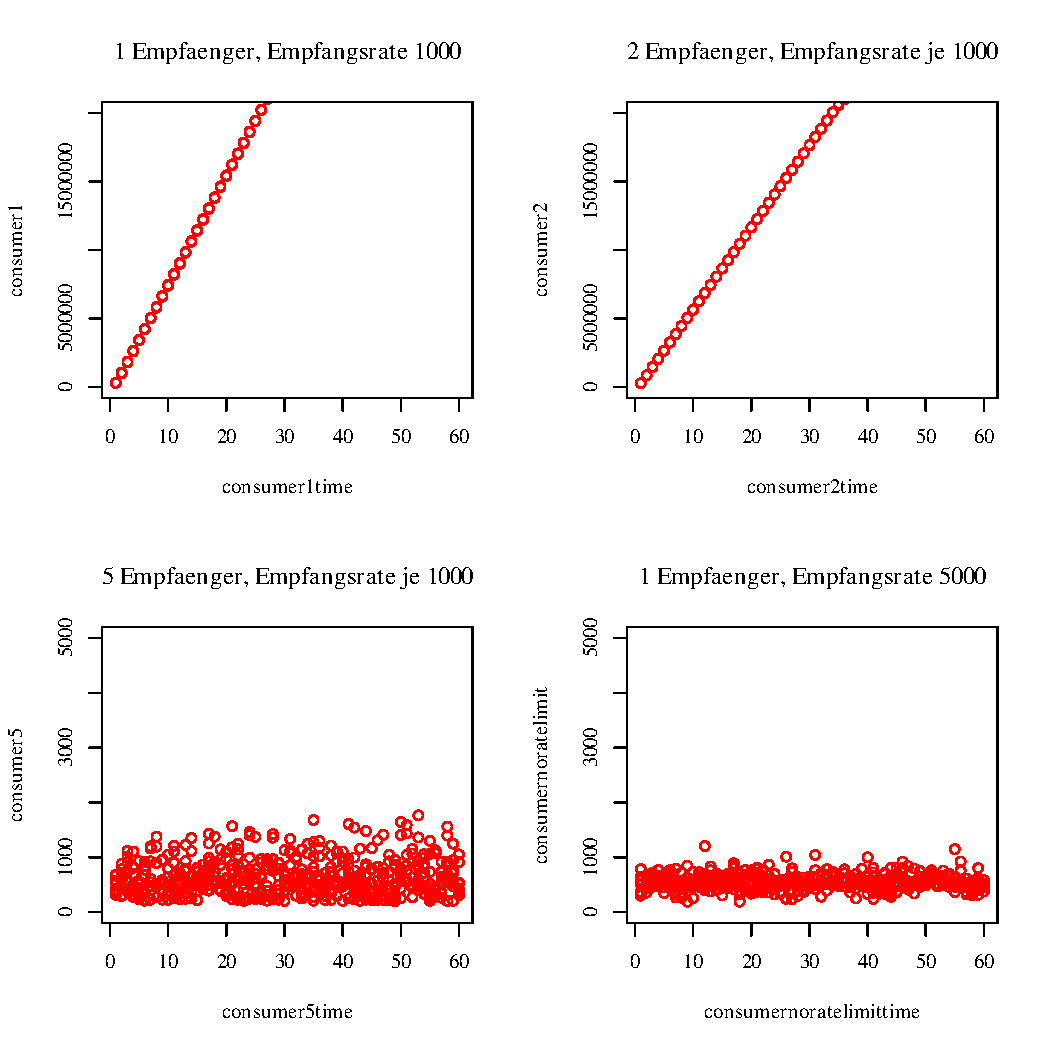
\includegraphics[width=0.7\textwidth]{images/measurement/varying-consumer.pdf}
  \caption{Verschiedene Empfaenger Anzahl}
  \label{img:varyingConsumer}
\end{figure}
%E
Diese stärkere Streuung lässt sich mit der Synchronisation der Empfänger erklären, die an einer gemeinsamen Warteschlange arbeiten. Da diese Streuung nicht stark ist, wird dieser Effekt im Folgenden vernachläßigt. Somit zeigt diese Messung, dass mehrere Empfänger gemeinsam an die Leistung eines einzelnen Empfängers heran kommen. 

\subsubsection{Mehrere Sender}
Diese Messung soll überprüfen, ob mehrere Sender genau so schnell die gleiche Menge an Nachrichten versenden können, wie ein einzelner. Dazu wurde als Referenz ein Sender mit einer Senderate von 5000 Nachrichten die Sekunde und fünf Sender mit jeweils 1000 Nachrichten die Sekunde untersucht. Die Messung wurde mit dem \textit{lokal}-Szenario durchgeführt. Erwartet wird, dass es keinen Unterschied macht, ob ein Sender 5000 Nachrichten sendet oder fünf Sender jeweils 1000 Nachrichten senden. 
%B
In \autoref{img:varyingProducer} sind die Ergebnisse dieser Messung zu sehen. Dabei ist zu sehen, dass mehr Sender etwas schlechter abschneiden als ein einzelner. 
\begin{figure}
\center
  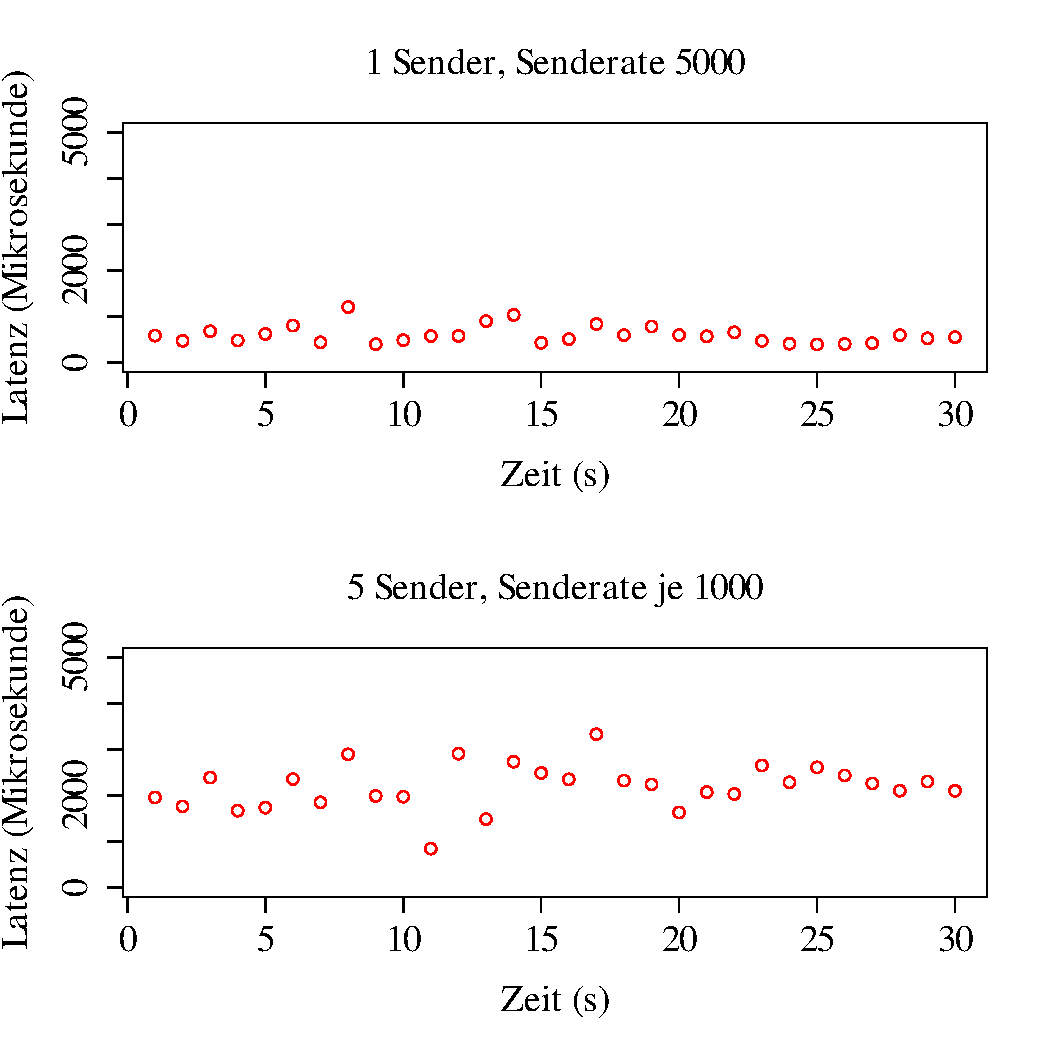
\includegraphics[width=0.7\textwidth]{images/measurement/varying-producer.pdf}
  \caption{Verschiedene Sender Anzahl}
  \label{img:varyingProducer}
\end{figure}
%E
Auch in diesem Fall kann die höhere Latenz, der mehreren Sender, auf die Synchronisation an einer Warteschlange zurückgeführt werden. Da jedoch dieser Effekt wieder im Mikrosekunden Bereich ist, wird dieser Effekt im Folgenden für die Modellierung vernachlässigt. 
%A
%In einer weiteren Messung sollte Ausserdem geprueft werden, ob mehrere Sender ohne Sendelimit mehr Nachrichten senden koennen als ein Sender. Dazu wurde der selbe Versuchsaufbau wie oben gewaehlt mit dem Unterschied, dass diesmal die Senderate nicht eingeschraenk wurde.
%B
%In \autoref{img:varyingProducerMaxThroughput} sind die Ergebnisse dargestellt. Dabei ist zu sehen, dass die 5 Sender zusammen genauso viele Nachrichten senden wie ein Sender allein. Ausserdem ist die Latenz im Fall der 5 Sender um ein 5faches groesser als bei einem Sender.
%\begin{figure}
%\center
%  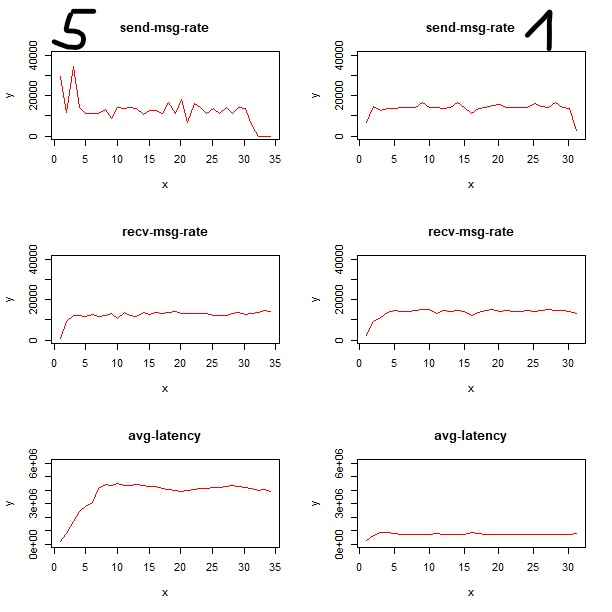
\includegraphics[width=1\textwidth]{images/varyingProducerMaxThroughput.jpg}
%  \caption{Verschiedene Sender Anzahl}
%  \label{img:varyingProducerMaxThroughput}
%\end{figure}
%E
%Das die 5 Sender jeweils nur 1/5 der moeglichen Senderate senden, kann dadurch erklaert werden, dass das Testsystem nicht mehr als eine bestimmte Rate an Nachrichten senden kann. D.h. das es keinen Unterschied macht ob ein Sender oder mehrere Sender Nachrichten senden. DIeses Verhalten kann sich aendern, wenn sich verschiedene Sender auf verschiedenen Maschinen befinden. (evtl noch Messung durchfuehren um zu zeigen) 


%Ableitung von ResourceDemands -> Regressionsfkt

%\subsection{ActiveMQ}
%ActiveMQ \cite{activeMQ} ist eine Open-Source-MOM, die seit 2004 kontinuierlich weiter entwickelt wird. ActiveMQ ist in Java geschrieben und implementiert den Java Message Service (JMS) \cite{jms}. Dabei handelt es sich um eine Programmierschnittstelle zur Ansteuerung einer MOM. Dabei soll eine lose gekoppelte, verlässliche und asynchrone Kommunikation zwischen den Komponenten einer verteilten Anwendung ermöglicht werden. ActiveMQ verfügt außerdem über mehrere Betriebsarten für hohe Verfügbarkeit und einen robusten horizontalen Skalierungsmechanismus. Darüber hinaus ist es sehr flexibel in der Konfiguration und unterstützt eine Vielzahl von Transportprotokollen, darunter auch AMQP.

\subsection{Zusammenfassung}
\label{sec:rmqZusammenfassung}
Mithilfe der durchgeführten Messungen konnten die folgenden Einflussfaktoren identifiziert werden, die einen Einfluss auf die Performance haben:
\begin{itemize}
    \item Die Nachrichtengröße hat einen Einfluss auf die Latenz einer Nachricht, die mögliche Senderate und die insgesamt gesendete Datenmenge.
    \item Die Netzwerklatenz zwischen Sender, Empfänger und Broker hat einen zusätzlichen Einfluss auf die Latenz einzelner Nachrichten.
    \item Die mögliche Datenmenge die auf einmal gesendet werden kann, ist durch die Netzwerkverbindung begrenzt.
    \item Wenn Nachrichten direkt aus der Warteschlange empfangen werden können, ist ihre Latenz gering.
    \item Die Latenz der Nachricht steigt, wenn die Warteschlange sich füllt und die Nachrichten in ihr warten müssen um abgeholt zu werden.
    \item Das Begrenzen der Warteschlangengröße kann die Latenz der Nachrichten klein halten.
    \item Ob Nachrichten in den Hauptspeicher oder auf die Festplatte geschrieben werden hat einen Einfluss auf die Latenz.
\end{itemize}
Mithilfe dieser Einflussfaktoren soll im Folgenden ein Modell einer MOM erstellt werden, mit dem diese Einflussfaktoren abgebildet werden können. Außerdem werden die Messergebnisse dieses Kapitels verwendet um das Modell zu kalibrieren.


%RMQ hat auch Prefetch von Nachrichten. Wird nicht betrachtet (zeit und trotzdem nicht so gut wie kafka) \\
%Latenz steigt an, wenn die queue gefuellt wird \\
%- benoetigt tracken einer Nachricht durch das system \\
%- explizite Queue Modellierung, mit groesse und fuellstand \\


%--	Vergleich: https://stackshare.io/stackups/activemq-vs-kafka-vs-rabbitmq  \\


